\chapter{ejercicio 3}
\part{Ejercicio 3}
\section{Enunciado}
Dado un arreglo de n elementos en el que hay un elemento que aparece m'as de la mitad de las veces, encontrar la moda, es
decir, el valor que aparece m'as veces.

\section{Desarrollo}
La primera idea para abordar este problema fue ordenar el arreglo y contar la cantidad de apariciones guardando el elemento con mas apariciones.
\paragraph{}
Una mejora a este procedimiento es notar que la moda en un arreglo con la caracteristica de los del problema, es decir que la 
moda esta mas de la mitad de las veces, coincide con el elemento n/2. Entonces si ordenamos el arreglo, en 
vez de contar apariciones podemos solamente tomar el elemento n/2  para obtener la moda. Ambos algoritmos tienen un orden n * 
log n, por lo que nos gustaria poder bajar ese orden. Investigando sobre el tema encontramos el algoritmo de 
Loyd-Pratt-Rivest-Tarjan que permite encontrar la mediana de un arreglo en orden lineal, sin necesidad de ordenarlo. La idea es 
usar un pivote para partir el arreglo y quedarnos solo con la parte donde puede estar la mediana. Es necesario para tener orden 
lineal poder encontrar un buen pivote en un orden a lo sumo lineal. El algoritmo resuelve esto partiendo el arreglo en arreglos 
de 5 elementos, tomando la mediana de estos y luego tomando la pseudomediana de estas ``mediana''.  Se puede demostrar que este 
procedimiento permite encontrar la mediana en orden lineal. Esta solucion se descarto por varias razones: En primer lugar su 
implementaci'on era bastante complicada. Por otro lado, la demostraci'on del orden es compleja.
\paragraph{}
Buscamos entonces otra forma de  obtener un orden lineal aprovechando que la frecuencia de la moda era mayor a la mitad. La idea basicamente es recorrer el  arreglo con dos indices. Si encontramos dos elementos iguales incrementamos uno de los indices (en adelante j) y dejamos al otro (en adelante i) en la posici'on donde esta. Si encontramos 2 elementos diferentes, los tachamos (ponemos una marca en un arreglo de booleanos). Luego avanzamos  i hasta que llegue a una posicion sin tachar y hacemos lo propio con j hasta llegar a una posicion sin tachar pero que tambien sea mayor que i. El ciclo termin cuando j se pasa del largo del arreglo. Entonces devolvemos el indice donde quedo parado el indice i.En cada paso el algoritmo ``tacha'' dos elementos que no son la moda, o uno que es la moda y otro que no. Entonces solo terminan sobreviviendo algunos elementos de la moda. Al terminar el ciclo, los elementos sin tachar desde i hasta el final del arreglo son iguales. Entonces podrian ser moda o elementos distintos a la moda. Esto ultimo no puede ocurrir ya que la frecuencia de la moda es como minimo n/2 + 1, entonces que ocurra  implicaria que tache por lo menos 2(n/2+1) $>$ n. Este algoritmo fue finalmente el que adoptamos como solucion ya que nos daba el orden lineal buscado y su implementacion era simple.

\section{Pseudocodigo}
\begin{algorithm}
\caption{Halla la moda $moda$ del arreglo $a$}
\begin{algorithmic}[1]
\STATE indiceDeAtras $\textcolor{orange}{\leftarrow}$ 0
\STATE indiceDeAdelante $\textcolor{orange}{\leftarrow}$ 0
\STATE tachados: [bool] \COMMENT{los elementos de tachados inicializan en false}\\

\WHILE{indiceDeAdelante $\textcolor{orange}{<}$ tamanio\textcolor{magenta}{(}a\textcolor{magenta}{)}}
    \IF{$a_{indiceDeAtras}$ $\textcolor{orange}{\neq}$ $a_{indiceDeAdelante}$}
        \STATE tachados $\textcolor{orange}{\leftarrow}$ tachar ambos elementos //donde: tachar i es asignar con true en el elemento iesimo de tachados
        \WHILE{\textcolor{magenta}{(}indiceDeAtras $\textcolor{orange}{<}$ tamanio\textcolor{magenta}{(}a\textcolor{magenta}{)} \textcolor{orange}{\&} \textcolor{magenta}{(}indiceDeAtras no fue tachado\textcolor{magenta}{)}}
            \STATE indiceDeAtras $\textcolor{orange}{\leftarrow}$ indiceDeAtras \textcolor{orange}{+} 1
        \ENDWHILE
        \WHILE{indiceDeAdelante $\textcolor{orange}{<}$ tamanio\textcolor{magenta}{(}a\textcolor{magenta}{)} \textcolor{orange}{\&} \textcolor{magenta}{(}indiceDeAdelante no fue tachado $\textcolor{orange}{|}$ indiceDeAdelante $\leq$ indiceDeAtras\textcolor{magenta}{)}}
            \STATE indiceDeAdelante $\textcolor{orange}{\leftarrow}$ indiceDeAdelante \textcolor{orange}{+} 1
        \ENDWHILE
    \ELSE
        \STATE indiceDeAdelante $\textcolor{orange}{\leftarrow}$ indiceDeAdelante \textcolor{orange}{+} 1
    \ENDIF

\ENDWHILE
\STATE $moda \textcolor{orange}{\leftarrow}$ $a_{indiceDeAtras}$
\end{algorithmic}
\end{algorithm}


\section{C'alculo de complejidad}

\section{Analisis Experimental}
\subsection{Experiencias realizadas}
Nuevamente para este algoritmo decidimos medir tanto la cantidad de operaciones como el tiempo, en funcion de la cantidad de 
elementos del arreglo con la intencion de confirmar nuestro analisis teorico. Para ello generamos arreglos de largo creciente 
con elementos al azar (distribuci'on uniforme) respetando que la frecuencia de la moda sea de por lo menos $n/2 + 1$\\
Por otro lado para observer la influencia de la frecuencia de la moda en el comportamiento del algoritmo realizamos corridas 
para un n fijo aumentando la frecuencia y midiendo la cantidad de operaciones y el tiempo.\\
En algunos casos ademas fue posible utilizando la tecnica de minimos cuadrados, dar una funcion que se aproxime al comportamiento obtenido experimentalmente. En dichos casos, la ecuacion de f(x) se encuentra en el grafico.

\subsection{Gr'aficos}
%TODO: rehacer estos graficos es al pedo tener 10^-5 segundos, pasar a milisegundos por lo menos 
\begin{figure}[H]
\centering
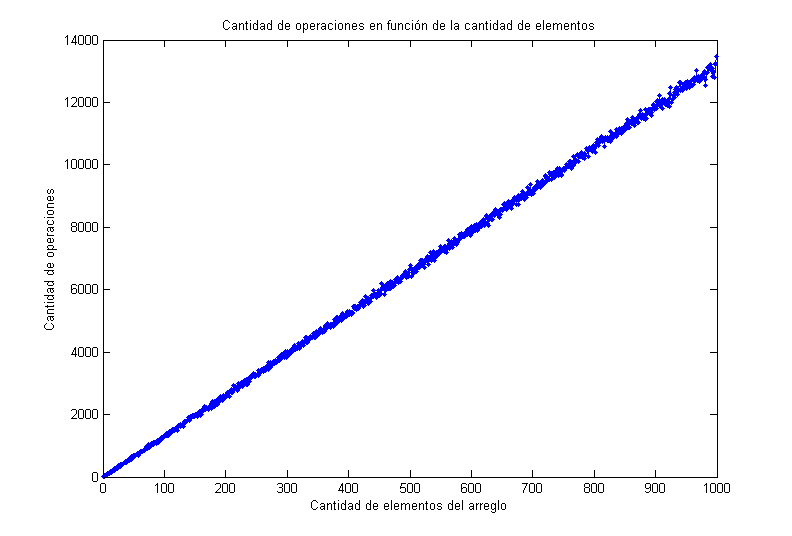
\includegraphics[scale=0.5]{../../codigo/ejercicio3/benchmark/graficos/corridas_aleatorias_n_creciente/grafico.png}
\caption{Cantidad de operaciones en funcion del tama\~{n}o del arreglo}
\end{figure}

\begin{figure}[H]
\centering
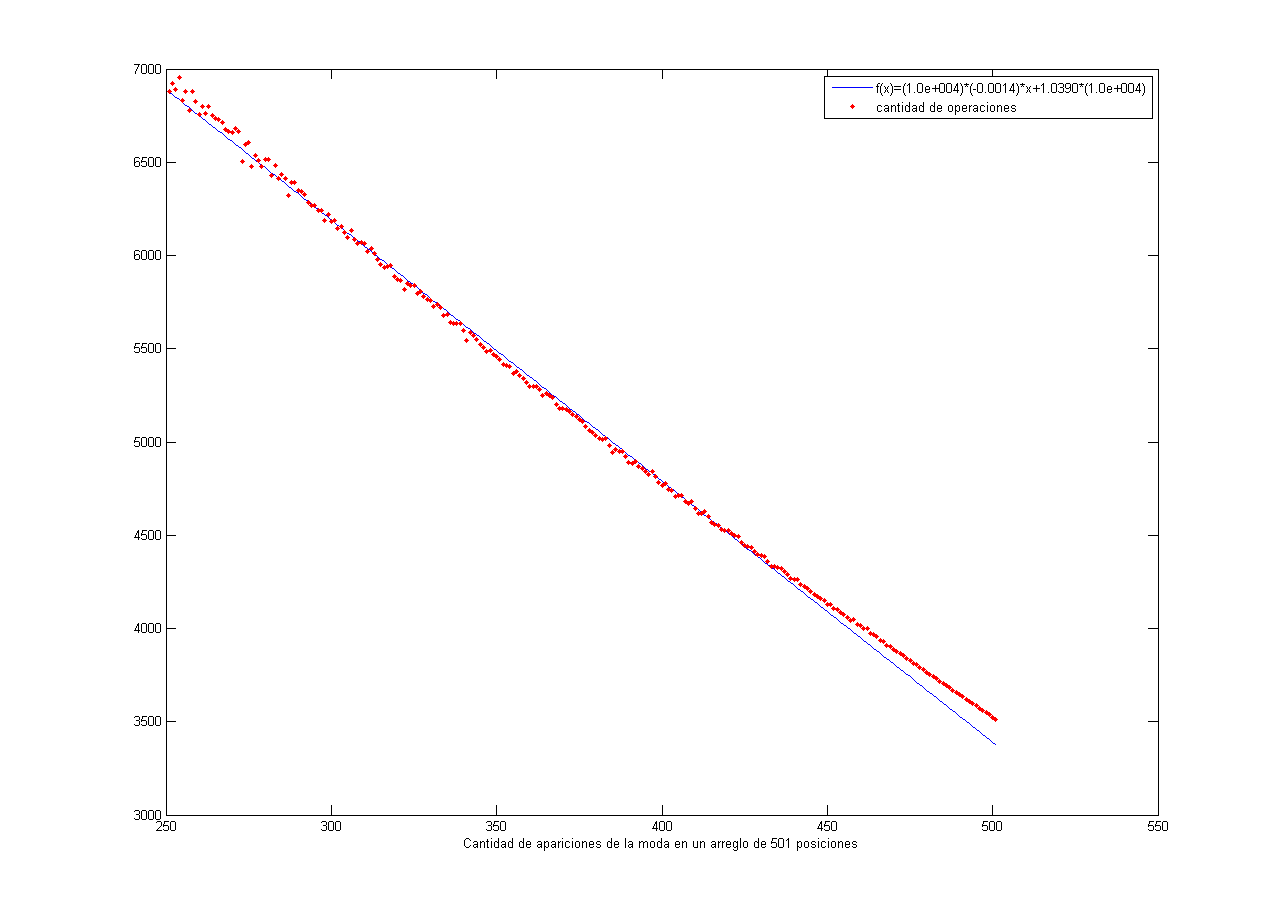
\includegraphics[scale=0.5]{../../codigo/ejercicio3/benchmark/graficos/frecuencia/frecuencia.png}
\caption{Cantidad de operaciones en funcion de la frecuencia (n = 501)}
\end{figure}

\begin{figure}[H]
\centering
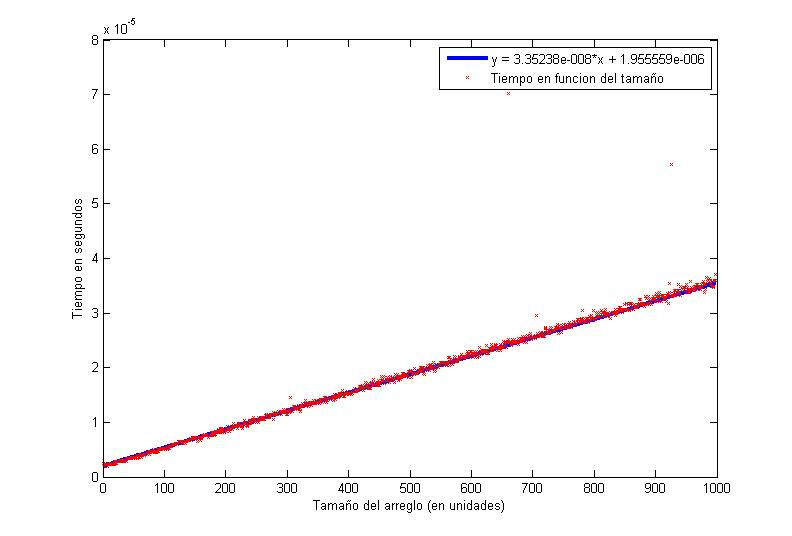
\includegraphics[scale=0.5]{../../codigo/ejercicio3/benchmark_de_tiempo/graficos/moda-1000-casos.jpg}
%TODO: rehacer este grafico es al pedo tener 10^-5 segundos, pasar a milisegundos por lo menos 
\caption{Tiempo (segundos) en funcion del tama\~{n}o del arreglo}
\end{figure}

\begin{figure}[H]
\centering
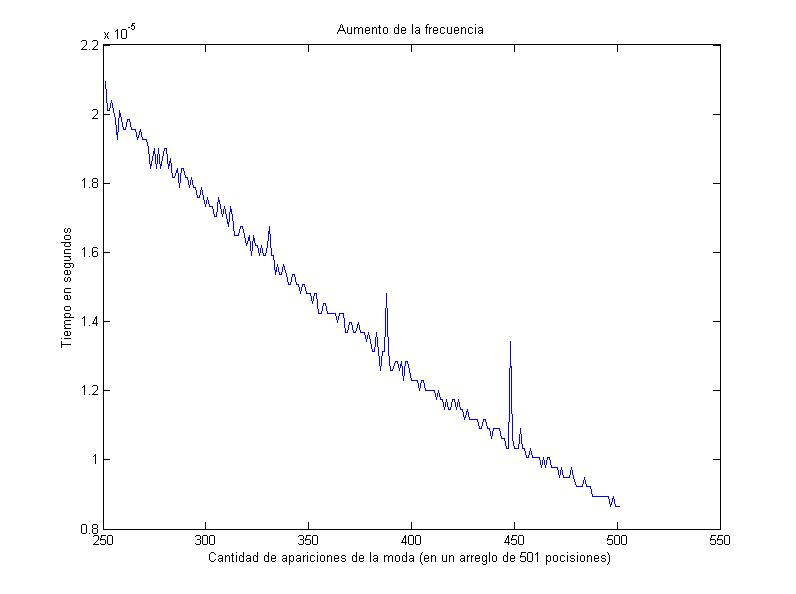
\includegraphics[scale=0.5]{../../codigo/ejercicio3/benchmark_de_tiempo/graficos/aumento-frecuencia.jpg}
\caption{Tiempo (segundos) en funcion de la frecuencia (n = 501)}
\end{figure}

\section{Discusi'on}
Tanto en los graficos de tiempo observamos que al aumentar el tama\~{n}o del arreglo el tiempo aumenta de forma lineal. Lo mismo ocurre con la cantidad de operaciones. Esta situacion se corresoponde con el analisis teorico que realizamos.
Por otro lado en los graficos en funcion de la frecuencia de la moda, el tiempo y las operaciones parecieran decrecer linealmente. Esto nos muestra que el mejor caso es cuando todos los elementos del arreglo son la moda. Esto se explica de la siguiente manera: si todos los elementos son iguales a la moda, el if de la linea 5 es siempre falso por lo que el ciclo recorre el arreglo sin hacer otro tipo de operacion.
